\documentclass[parskip=half]{scrartcl}
        \usepackage{tikz}
        \usepackage{pxfonts}
        \usepackage[a4paper,left=1cm,right=1cm,top=2cm,bottom=3cm]{geometry}
        \title{Conformance Testing Report}
        \author{\relax}\date{\today}
        \begin{document} \maketitle
        \section{Benchmark information}This part has been removed for the moment.\section{{Predictor Information}}\subsection{Conformance Predictor 0 }Quantile-Cell THR Conformal Prediction: rotated views define a frozen quantile partition with ? possible ranges. Each range owns a distinct THR split-conformal predictor and is calibrated only with calibration samples routed to that range. Prediction uses the range-specific finite-sample conformal threshold; ranges with insufficient calibration mass use the conservative full-set threshold.\subsection{Conformance Predictor 1 }No-TTA (leading views) + THR\section{Direct comparison between all conformance prediction approaches}
The following comparison shows the performance of different conformance predictors. The X Axis shows the needed precision, while the Y axis shows, for each conformance prediction approach, precision on the conformance calibration set and the resulting mean conformance set sizes.

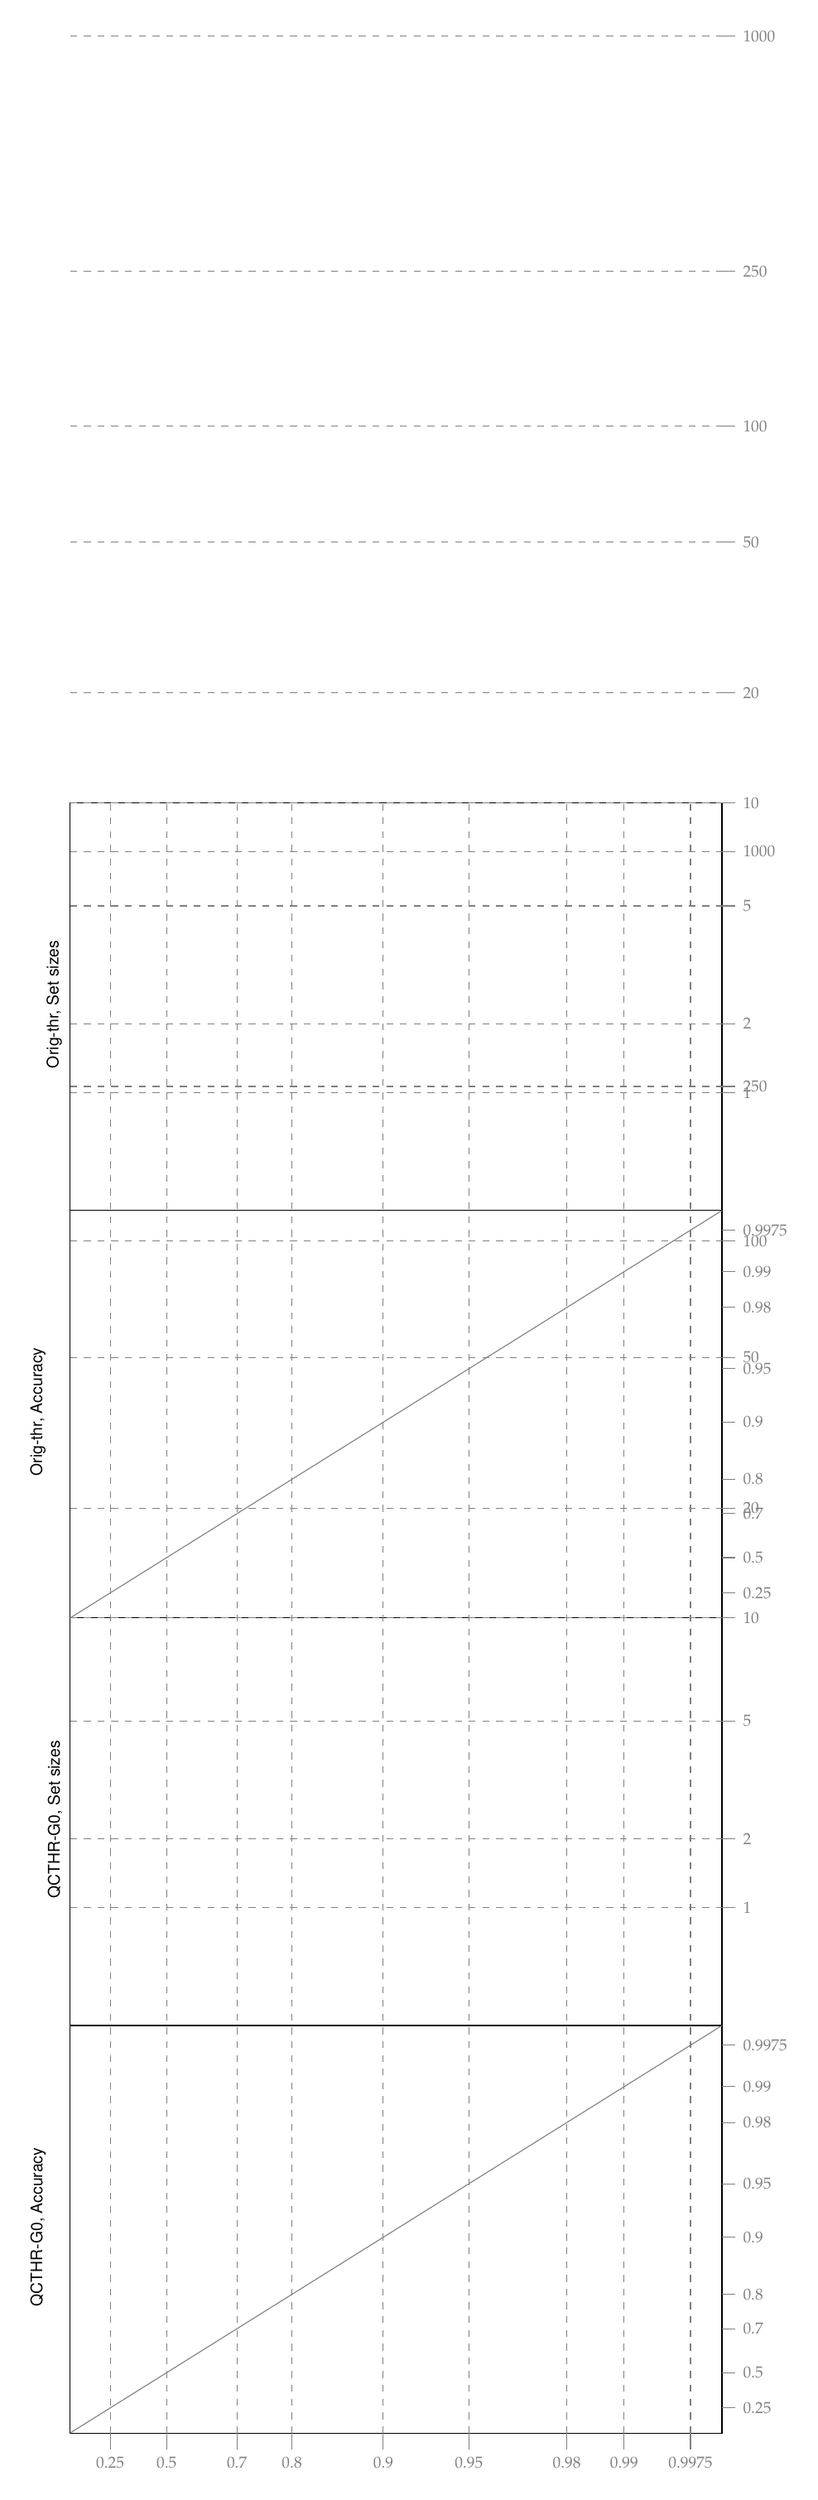
\begin{tikzpicture}[yscale=1.25]\draw (0,0) rectangle (10,20);
\draw (0,5) -- +(10,0);\draw (0,10) -- +(10,0);\node[anchor=east] at (-0.25,2.5) {\rotatebox{90}{\scriptsize \textsf{ QCTHR-G0, Accuracy}}};
\node[anchor=east] at (0,7.5) {\rotatebox{90}{\scriptsize \textsf{ QCTHR-G0, Set sizes}}};
\draw (0,15) -- +(10,0);\node[anchor=east] at (-0.25,12.5) {\rotatebox{90}{\scriptsize \textsf{ Orig-thr, Accuracy}}};
\node[anchor=east] at (0,17.5) {\rotatebox{90}{\scriptsize \textsf{ Orig-thr, Set sizes}}};
\draw[color=black!50!white] (0,0) -- +(10,5);
\draw[color=black!50!white] (0,10) -- +(10,5);
\draw[color=black!50!white] (0.6162074760933258,0) -- +(0,-0.2) node[below] {\scriptsize 0.25};
\draw[color=black!50!white,dashed] (0.6162074760933258,0) -- +(0,20);
\draw[color=black!50!white] (1.4805569683900757,0) -- +(0,-0.2) node[below] {\scriptsize 0.5};
\draw[color=black!50!white,dashed] (1.4805569683900757,0) -- +(0,20);
\draw[color=black!50!white] (2.5592686215798315,0) -- +(0,-0.2) node[below] {\scriptsize 0.7};
\draw[color=black!50!white,dashed] (2.5592686215798315,0) -- +(0,20);
\draw[color=black!50!white] (3.4031572380103423,0) -- +(0,-0.2) node[below] {\scriptsize 0.8};
\draw[color=black!50!white,dashed] (3.4031572380103423,0) -- +(0,20);
\draw[color=black!50!white] (4.804262935175594,0) -- +(0,-0.2) node[below] {\scriptsize 0.9};
\draw[color=black!50!white,dashed] (4.804262935175594,0) -- +(0,20);
\draw[color=black!50!white] (6.117632329015766,0) -- +(0,-0.2) node[below] {\scriptsize 0.95};
\draw[color=black!50!white,dashed] (6.117632329015766,0) -- +(0,20);
\draw[color=black!50!white] (7.619537161252646,0) -- +(0,-0.2) node[below] {\scriptsize 0.98};
\draw[color=black!50!white,dashed] (7.619537161252646,0) -- +(0,20);
\draw[color=black!50!white] (8.49809516776312,0) -- +(0,-0.2) node[below] {\scriptsize 0.99};
\draw[color=black!50!white,dashed] (8.49809516776312,0) -- +(0,20);
\draw[color=black!50!white] (9.516494638655868,0) -- +(0,-0.2) node[below] {\scriptsize 0.9975};
\draw[color=black!50!white,dashed] (9.516494638655868,0) -- +(0,20);
\draw[color=black!50!white] (10,0.3081037380466629) -- +(0.2,0) node[right] {\scriptsize 0.25};
\draw[color=black!50!white] (10,0.7402784841950378) -- +(0.2,0) node[right] {\scriptsize 0.5};
\draw[color=black!50!white] (10,1.2796343107899157) -- +(0.2,0) node[right] {\scriptsize 0.7};
\draw[color=black!50!white] (10,1.7015786190051712) -- +(0.2,0) node[right] {\scriptsize 0.8};
\draw[color=black!50!white] (10,2.402131467587797) -- +(0.2,0) node[right] {\scriptsize 0.9};
\draw[color=black!50!white] (10,3.058816164507883) -- +(0.2,0) node[right] {\scriptsize 0.95};
\draw[color=black!50!white] (10,3.809768580626323) -- +(0.2,0) node[right] {\scriptsize 0.98};
\draw[color=black!50!white] (10,4.24904758388156) -- +(0.2,0) node[right] {\scriptsize 0.99};
\draw[color=black!50!white] (10,4.758247319327934) -- +(0.2,0) node[right] {\scriptsize 0.9975};
\draw[color=black!50!white,dashed] (0,6.445324131589439) -- +(10,0);
\draw[color=black!50!white] (10,6.445324131589439) -- +(0.2,0) node[right] {\scriptsize 1};
\draw[color=black!50!white,dashed] (0,7.29078454995663) -- +(10,0);
\draw[color=black!50!white] (10,7.29078454995663) -- +(0.2,0) node[right] {\scriptsize 2};
\draw[color=black!50!white,dashed] (0,8.736108681546071) -- +(10,0);
\draw[color=black!50!white] (10,8.736108681546071) -- +(0.2,0) node[right] {\scriptsize 5};
\draw[color=black!50!white,dashed] (0,10.0) -- +(10,0);
\draw[color=black!50!white] (10,10.0) -- +(0.2,0) node[right] {\scriptsize 10};
\draw[color=black!50!white,dashed] (0,11.348322364742875) -- +(10,0);
\draw[color=black!50!white] (10,11.348322364742875) -- +(0.2,0) node[right] {\scriptsize 20};
\draw[color=black!50!white,dashed] (0,13.198493231390879) -- +(10,0);
\draw[color=black!50!white] (10,13.198493231390879) -- +(0.2,0) node[right] {\scriptsize 50};
\draw[color=black!50!white,dashed] (0,14.623273729247071) -- +(10,0);
\draw[color=black!50!white] (10,14.623273729247071) -- +(0.2,0) node[right] {\scriptsize 100};
\draw[color=black!50!white,dashed] (0,16.52146426454129) -- +(10,0);
\draw[color=black!50!white] (10,16.52146426454129) -- +(0.2,0) node[right] {\scriptsize 250};
\draw[color=black!50!white,dashed] (0,19.405872636907585) -- +(10,0);
\draw[color=black!50!white] (10,19.405872636907585) -- +(0.2,0) node[right] {\scriptsize 1000};
\draw[color=black!50!white] (10,10.308103738046663) -- +(0.2,0) node[right] {\scriptsize 0.25};
\draw[color=black!50!white] (10,10.740278484195038) -- +(0.2,0) node[right] {\scriptsize 0.5};
\draw[color=black!50!white] (10,11.279634310789916) -- +(0.2,0) node[right] {\scriptsize 0.7};
\draw[color=black!50!white] (10,11.701578619005172) -- +(0.2,0) node[right] {\scriptsize 0.8};
\draw[color=black!50!white] (10,12.402131467587797) -- +(0.2,0) node[right] {\scriptsize 0.9};
\draw[color=black!50!white] (10,13.058816164507883) -- +(0.2,0) node[right] {\scriptsize 0.95};
\draw[color=black!50!white] (10,13.809768580626322) -- +(0.2,0) node[right] {\scriptsize 0.98};
\draw[color=black!50!white] (10,14.24904758388156) -- +(0.2,0) node[right] {\scriptsize 0.99};
\draw[color=black!50!white] (10,14.758247319327934) -- +(0.2,0) node[right] {\scriptsize 0.9975};
\draw[color=black!50!white,dashed] (0,16.445324131589437) -- +(10,0);
\draw[color=black!50!white] (10,16.445324131589437) -- +(0.2,0) node[right] {\scriptsize 1};
\draw[color=black!50!white,dashed] (0,17.29078454995663) -- +(10,0);
\draw[color=black!50!white] (10,17.29078454995663) -- +(0.2,0) node[right] {\scriptsize 2};
\draw[color=black!50!white,dashed] (0,18.73610868154607) -- +(10,0);
\draw[color=black!50!white] (10,18.73610868154607) -- +(0.2,0) node[right] {\scriptsize 5};
\draw[color=black!50!white,dashed] (0,20.0) -- +(10,0);
\draw[color=black!50!white] (10,20.0) -- +(0.2,0) node[right] {\scriptsize 10};
\draw[color=black!50!white,dashed] (0,21.348322364742877) -- +(10,0);
\draw[color=black!50!white] (10,21.348322364742877) -- +(0.2,0) node[right] {\scriptsize 20};
\draw[color=black!50!white,dashed] (0,23.198493231390877) -- +(10,0);
\draw[color=black!50!white] (10,23.198493231390877) -- +(0.2,0) node[right] {\scriptsize 50};
\draw[color=black!50!white,dashed] (0,24.62327372924707) -- +(10,0);
\draw[color=black!50!white] (10,24.62327372924707) -- +(0.2,0) node[right] {\scriptsize 100};
\draw[color=black!50!white,dashed] (0,26.52146426454129) -- +(10,0);
\draw[color=black!50!white] (10,26.52146426454129) -- +(0.2,0) node[right] {\scriptsize 250};
\draw[color=black!50!white,dashed] (0,29.405872636907585) -- +(10,0);
\draw[color=black!50!white] (10,29.405872636907585) -- +(0.2,0) node[right] {\scriptsize 1000};
\end{tikzpicture}\section{Interesting cases found Calibration}
\textbf{Cases filtered:} Interesting cases with large deviation for target probability 0.99


\textbf{Parameter/Probability Combinations considered:}\begin{enumerate}
\item (none)
\end{enumerate}\section{Performance on test data}
\paragraph{Predictor:QCTHR-G2} calibration at alpha=0.01. calibration value={0: 0.9995139544869237, 1: 0.9999556537183238}. Correct: 2467/2500\\
Average set size: 3.2736   Coverage: 0.9868\\
Set size histogram (0..K):\\
0 | 846 | 421 | 308 | 242 | 201 | 153 | 113 | 96 | 78 | 42\\
\paragraph{Metrics for QCTHR-G2}~\\
\begin{tabular}{l r}
\hline
Coverage (target 0.990) & 0.9868 $\pm$ 0.0023 \\
Average set size & 3.274 \\
Median set size & 2.0 \\
Singleton rate (size $=1$) & 0.3384 \\
Large-set rate (size $\geq 3$) & 0.4932 \\
\textbf{SSCV} (worst size-bin gap) & \textbf{0.0133} \\
Class-coverage spread (max$-$min) & 0.0347 \\
Class-coverage std & 0.0091 \\
\textbf{CovGap} (difficulty-conditioned) & \textbf{0.0084} \\
~~Weighted CovGap & 0.0084 \\
~~Worst under-coverage & -0.0260 \\
\hline
\end{tabular}\\[0.5em]
\textsf{\scriptsize Size-stratified coverage (SSCV bins):}\\
\begin{tabular}{l r r}
\hline
Size range & Count & Coverage \\
\hline
1 & 846 & 0.9905 \\
2--3 & 729 & 0.9767 \\
4--6 & 596 & 0.9899 \\
7--10 & 329 & 0.9939 \\
\hline
\end{tabular}\\[0.5em]
\textsf{\scriptsize Difficulty-stratified coverage (CovGap bins, by $1-\max p_{\mathrm{orig}}$):}\\
\begin{tabular}{l r r}
\hline
Difficulty range & Count & Coverage \\
\hline
0.000--0.000 & 250 & 0.9920 \\
0.000--0.000 & 250 & 0.9960 \\
0.000--0.000 & 250 & 0.9880 \\
0.000--0.000 & 250 & 0.9640 \\
0.000--0.001 & 250 & 0.9720 \\
0.001--0.004 & 250 & 0.9840 \\
0.004--0.022 & 250 & 1.0000 \\
0.022--0.084 & 250 & 0.9960 \\
0.084--0.266 & 250 & 0.9920 \\
0.266--0.680 & 250 & 0.9840 \\
\hline
\end{tabular}\\[0.5em]
\paragraph{Predictor:Orig-thr} calibration at alpha=0.01. calibration value=0.999932087803147. Correct: 2470/2500\\
Average set size: 3.2616   Coverage: 0.988\\
Set size histogram (0..K):\\
0 | 913 | 412 | 268 | 218 | 192 | 139 | 118 | 96 | 87 | 57\\
\paragraph{Metrics for Orig-thr}~\\
\begin{tabular}{l r}
\hline
Coverage (target 0.990) & 0.9880 $\pm$ 0.0022 \\
Average set size & 3.262 \\
Median set size & 2.0 \\
Singleton rate (size $=1$) & 0.3652 \\
Large-set rate (size $\geq 3$) & 0.4700 \\
\textbf{SSCV} (worst size-bin gap) & \textbf{0.0062} \\
Class-coverage spread (max$-$min) & 0.0309 \\
Class-coverage std & 0.0085 \\
\textbf{CovGap} (difficulty-conditioned) & \textbf{0.0084} \\
~~Weighted CovGap & 0.0084 \\
~~Worst under-coverage & -0.0260 \\
\hline
\end{tabular}\\[0.5em]
\textsf{\scriptsize Size-stratified coverage (SSCV bins):}\\
\begin{tabular}{l r r}
\hline
Size range & Count & Coverage \\
\hline
1 & 913 & 0.9869 \\
2--3 & 680 & 0.9838 \\
4--6 & 549 & 0.9909 \\
7--10 & 358 & 0.9944 \\
\hline
\end{tabular}\\[0.5em]
\textsf{\scriptsize Difficulty-stratified coverage (CovGap bins, by $1-\max p_{\mathrm{orig}}$):}\\
\begin{tabular}{l r r}
\hline
Difficulty range & Count & Coverage \\
\hline
0.000--0.000 & 250 & 0.9920 \\
0.000--0.000 & 250 & 0.9960 \\
0.000--0.000 & 250 & 0.9880 \\
0.000--0.000 & 250 & 0.9640 \\
0.000--0.001 & 250 & 0.9720 \\
0.001--0.004 & 250 & 0.9840 \\
0.004--0.022 & 250 & 1.0000 \\
0.022--0.084 & 250 & 0.9960 \\
0.084--0.266 & 250 & 0.9960 \\
0.266--0.680 & 250 & 0.9920 \\
\hline
\end{tabular}\\[0.5em]
\subsection{Metric comparison across predictors}
\begin{tabular}{l r r r r r r r r}
\hline
Predictor & Coverage & Avg size & Median & Singleton & Large & SSCV & CovGap & wUnder \\
\hline
QCTHR-G2 & 0.9868 & 3.274 & 2.0 & 0.3384 & 0.4932 & 0.0133 & 0.0084 & -0.0260 \\
Orig-thr & 0.9880 & 3.262 & 2.0 & 0.3652 & 0.4700 & 0.0062 & 0.0084 & -0.0260 \\
\hline
\end{tabular}\\[0.5em]
\textsf{\scriptsize SSCV = worst absolute coverage gap across prediction-set-size strata. CovGap = mean absolute deviation of difficulty-stratified coverage from the target $1-\alpha$. wUnder = worst difficulty-stratum under-coverage; values closer to zero are better.}\\
\section{Interesting cases found Testing}
\textbf{Cases filtered:} Interesting cases with large deviation for target probability 0.99


\textbf{Parameter/Probability Combinations considered:}\begin{enumerate}
\item (none)
\end{enumerate}
        \end{document}
        